

%!TEX TS-program = xelatex
%!TEX encoding = UTF-8 Unicode


\documentclass[12pt]{scrartcl}

\usepackage{tipa}
\usepackage{xunicode,xltxtra, polyglossia}
\usepackage{fontspec} 
\usepackage[round]{natbib}
\DeclareTextCommandDefault{\nobreakspace}{\leavevmode\nobreak\ } 

\usepackage{array}
\usepackage{gb4e}


\setmainfont[Ligatures={Common},ItalicFont = Linux Libertine O Italic]{Linux Libertine O}
\setsansfont[Scale=MatchLowercase,Mapping=tex-text]{Optima}



\title{Amharic Geminates and a Potential Relation to Stress}
\subtitle{Phonetics Final Paper}
\author{Andrew Hedding and Lisa Hofmann}
\begin{document}
\renewcommand\textipa[1]{{\fontfamily{cmr}\tipaencoding #1}}

\maketitle
\section{Introduction}

In a recent paper, \cite{sande2017} argue that Amharic, a Semitic language spoken in Ethiopia, provides evidence to support a particular prediction of Moraic Theory. Specifically, they point to two phonological processes in the language---reduplication and stress assignment---which demonstrate that geminate codas are underlyingly moraic, while singleton codas are not. 

Moraic Theory hypothesizes that all geminates will contribute weight to syllables (\cite{hayes1989}). Singleton codas create heavy syllables in some languages when Weight-By-Position is activated. Thus the theory predicts that there should be languages where only geminate codas create a heavy syllable. Any language that has geminates, but where Weight-By-Position is inactive, should display that pattern. Sande and Hedding argue that Amharic is such a language based on two phonological processes. First, reduplication on adjectives to form plurals only targets words with geminates. For example:

\begin{exe}
\ex{Singular Form $\rightarrow$ Plural Form}
\begin{xlist}
\ex 	\textipa{tanna\textesh} $\rightarrow$ \textipa{ta\underline{na}nna\textesh} \hspace{1cm} `younger'
\ex 	\textipa{tallak'} $\rightarrow$ \textipa{ta\underline{la}llak'} \hspace{1.18cm} `older'
\ex 	\textipa{hajjal} $\rightarrow$ \textipa{ha\underline{ja}jjal} \hspace{1.37cm} `powerful'
\end{xlist}
\end{exe}

Adjectives without a geminate cannot undergo reduplication and instead are inflected with a plural suffix. 

\begin{exe}
\ex{Singular Form $\rightarrow$ Plural Form}
\begin{xlist}
\ex 	\textipa{kon\texttoptiebar{\textdyoghlig}o} $\rightarrow$ *\textipa{ko\underline{na}n\texttoptiebar{\textdyoghlig}o} 
\ex 	\textipa{kon\texttoptiebar{\textdyoghlig}o} $\rightarrow$ \textipa{kon\texttoptiebar{\textdyoghlig}o-o\texttoptiebar{\textteshlig}\texttoptiebar{\textteshlig}} \hspace{1cm} `beautiful'
\end{xlist}
\end{exe}

Geminates are reduplicated and infixed along with an epenthetic vowel. Sande and Hedding argue that this type of reduplication is only possible in words that have a geminate and that the reduplicated geminate surfaces as a singleton. 

Second, they claim that syllables closed by a geminate are always stressed. They use this phonological evidence to hypothesize that only syllables with geminate codas are heavy in the language, confirming a typological prediction made by Moraic Theory.

The aim of the present paper is to scrutinize the hypotheses of Sande and Hedding, using phonetic analysis to test their central claims. Specifically, we use recordings of reduplicated adjectives to test the relative length of the geminate and singleton consonant, and we use three well-known correlates of stress to determine whether the syllable closed by a geminate displays typical patterns associated with stress. In their paper, Sande and Hedding acknowledge that their data on geminates and stress patterns were mostly analyzed impressionistically, although they did check a few examples using Praat. This paper seeks to verify their analysis in a more systematic way, using phonetic measurements. 

The results of the present analysis clearly confirm that all test words that underwent reduplication had geminate consonants, when compared to the reduplicated singleton. The results don't clearly support, however, the claim that all syllables closed by a geminate are stressed. Data was gathered on three phonetic variables---duration, pitch, and intensity---which have been noted by \cite{hayes1995} and \cite{fox2002} to be cross-linguistically correlates of stress. The syllables predicted to be stressed by Sande and Hedding did not, on average, have longer durations or higher pitch, nor did they have a higher mean intensity. 

At this early stage, it seems one of the hypotheses of Sande and Hedding is not clearly supported by the phonetic evidence. This study contains a small amount of data, however, from only two speakers. In order to determine more conclusively whether the the stress pattern in Amharic is linked to the presence of geminates, more data must be collected from a wider variety of words and contexts, and it must be put through more sophisticated statistical analysis.

\section{Methodology}

Recordings were made of two native Amharic speakers, one female and one male, saying a series of adjectives that can grammatically undergo reduplication. They each recorded  8 and 9 words, respectively, 5 of which were identical to a word that the other had recorded, as well as several unique words each. This created a total of 15 total test words, which are given in table \textbf{\ref{tab:words}}. All words selected were three syllables long, and they had the same basic syllable structure---(C)V.CVG.GV(C)---where the second syllable is predicted to be stressed due to the fact that it is closed by a geminate. One word---\emph{\textipa{wufaffram}}---had an addition consonant at the beginning of the final syllable. This was analyzed as part of a complex onset with the preceding geminate. All recordings are of the reduplicated form of the word.

\begin{table}[h]
\caption{Recorded words by subject. The items that differed by speaker are highlighted in boldface \label{tab:words}}
\begin{center} \renewcommand*\arraystretch{1.2}
\scalebox{1}[1]{\begin{tabular}[t]{|rrl|c|} \hline
\multicolumn{3}{|c|}{\textbf{Male Speaker}} & \textbf{Female speaker} \\[0.5ex]
\hline & \textipa{a\texttoptiebar{\textteshlig}a\texttoptiebar{\textteshlig}\texttoptiebar{\textteshlig}\textbari r} & & \textipa{a\texttoptiebar{\textteshlig}a\texttoptiebar{\textteshlig}\texttoptiebar{\textteshlig}\textbari r} \\
\hline & \textipa{d\textepsilon mammak'} & & \textipa{d\textepsilon mammak'} \\
\hline & \textipa{r\textepsilon\texttoptiebar{\textdyoghlig}a\texttoptiebar{\textdyoghlig}\texttoptiebar{\textdyoghlig}\textbari m} & & \textipa{r\textepsilon\texttoptiebar{\textdyoghlig}a\texttoptiebar{\textdyoghlig}\texttoptiebar{\textdyoghlig}\textbari m} \\
\hline & \textipa{talallak'} & & \textipa{talallak'} \\
\hline & \textipa{tananna\textesh} & & \textipa{tananna\textesh} \\
\hline & \textbf{\textipa{adaddis}} & & \textbf{\textipa{hajajjal}} \\
\hline & \textbf{\textipa{ka\texttoptiebar{\textteshlig}a\texttoptiebar{\textteshlig}\texttoptiebar{\textteshlig}\textsyllabic{n}}} & & \textbf{\textipa{wufaffram}} \\
\hline & \textbf{\textipa{safaffi}} & & \\
\hline \end{tabular}} \renewcommand*\arraystretch{1} \end{center}
\end{table}


Recordings were annotated and analyzed using Praat. Words were split into segments and syllables in order to be measured. An example annotation is given in figure \textbf{\ref{fig:annotate}}. Words were syllabified under the assumption that onsets are cross-linguistically preferred over codas, thus any consonant that could be either a coda or an onset was analyzed as an onset. Because geminates are argued to function as both the coda of one syllable and the onset of the following syllable, geminates were split in half when assigned to syllables.

Recordings were annotated and analyzed using Praat. Words were split into segments and syllables in order to be measured. An example annotation is given in Figure (\ref{fig:annotate}):

\begin{figure}[h]
	\centering
	\caption{Example annotation in Praat \label{fig:annotate}}
	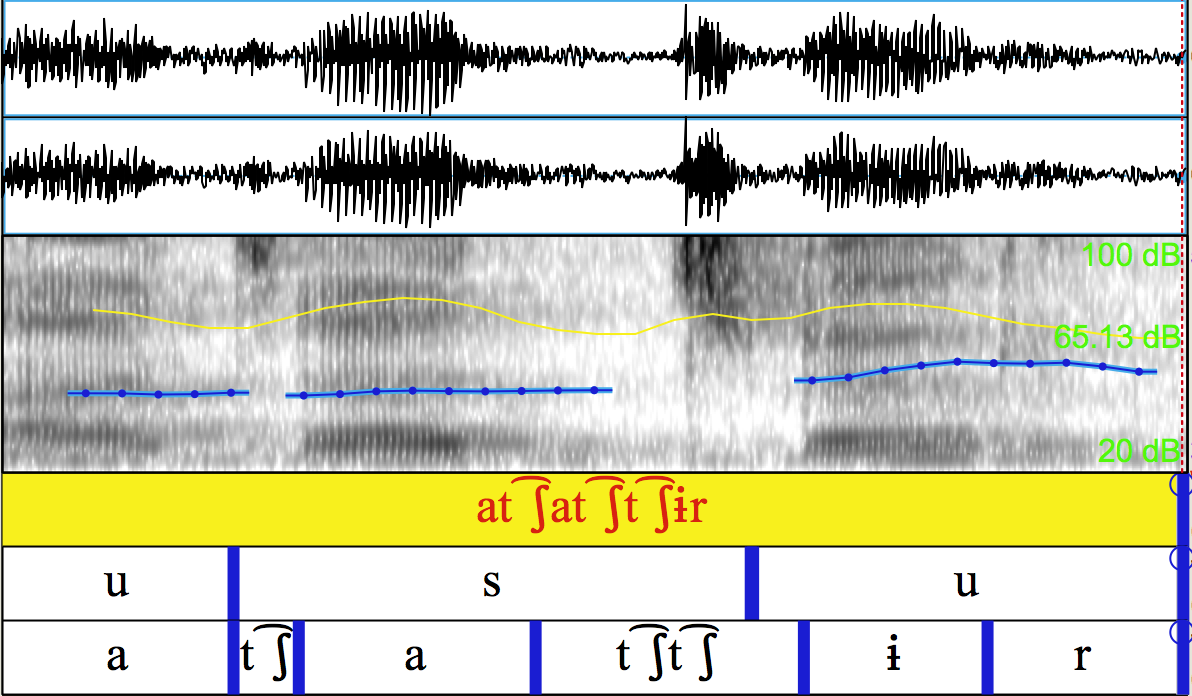
\includegraphics[width=.8\textwidth]{exann.png}
\end{figure}

In order to test the hypothesis that words with geminates undergo reduplication, we compared the duration of the reduplicated consonant and the base consonant. Using Praat, we measured the mean pitch in Hz and the mean intensity in dB of each syllable, as well as the duration of each syllable.

As an additional test, recordings of the female speaker were presented to the male speaker so he could judge the stress pattern impressionistically. Unfortunately the results of this test were inconclusive. The speaker consistently said that none of the syllables was stressed or more prominent than the others. This result seems consistent with the claim of \cite{hudson1997} that stress is not prominent in Amharic. The only syllable that he believed was stressed was the final syllable of \emph{\textipa{d\textepsilon mammak'}}. As that word has a final ejective consonant, it is likely that he associated the burst of energy that accompanies ejectives as prominence. The speaker said that changing the stress would not affect the meaning of the words, showing that he may have interpreted `stress' as only lexical stress. This seems to indicate that, at least for this speaker, words do not have an intuitively clear stress pattern in the language. We believe a more thorough study with more participants and clearer instructions about how to determine stress may be necessary to draw conclusions about how native speakers view the stress pattern of their language. 

\section{Results}
\subsection{Geminates and singletons in reduplication contexts}

\cite{sande2017} argue that the reduplicated adjectives involve a geminate in the reduplicant-base, whereas only a singleton consonant surfaces as part of the reduplicant. The phonetic plausibility of this analysis was tested by comparing the duration of the consonants analyzed as geminates to the duration of the consonants that are the result of the reduplication process.

The comparison across the two kinds of consonants was made by taking the mean duration of each group and comparing them. The consonant durations and mean consonant durations across base/reduplicant pairs by speaker are given in table \textbf{\ref{gemfemale}} for the female speaker and in table \textbf{\ref{gemmale}} for the male speaker.

\begin{table}[h]
	\caption{Consonant duration and mean consonant duration of female speaker in seconds (rounded to 4 digits) \label{gemfemale}}
	\centering
	\scalebox{1}[1]{\begin{tabular}[t]{|rrl|c|c|} \hline
		\multicolumn{3}{|c|}{Word} & \textbf{Singleton Duration} & \textbf{Geminate Duration} \\[0.5ex]
		\hline  \textipa{a\texttoptiebar{\textteshlig}a\texttoptiebar{\textteshlig}\texttoptiebar{\textteshlig}\textbari r} & & & 0.045 & 0.185  \\
		\hline  \textipa{d\textepsilon mammak'} & & & 0.113 & 0.169  \\
		\hline  \textipa{hajajjal} & & & 0.115 & 0.151 \\
		\hline  \textipa{r\textepsilon\texttoptiebar{\textdyoghlig}a\texttoptiebar{\textdyoghlig}\texttoptiebar{\textdyoghlig}\textbari m} & & & 0.093 & 0.189 \\
		\hline  \textipa{talallak'} & & & 0.057 & 0.131 \\
		\hline  \textipa{tananna\textesh} & & & 0.048 & 0.159 \\
		\hline  \textipa{wufaffram} & & & 0.082 & 0.111 \\
		\hline  \textbf{Mean Duration:} & & & \textbf{0.079 sec.} & \textbf{0.156 sec.} \\
		\hline
		\end{tabular}} \renewcommand*\arraystretch{1} 
\end{table}


\begin{table}[h]
	\caption{Consonant duration and mean consonant duration of male speaker in seconds (rounded to 4 digits) \label{gemmale}}
	\centering
	 \renewcommand*\arraystretch{1.2}
		\scalebox{1}[1]{\begin{tabular}[t]{|rrl|c|c|} \hline
		\multicolumn{3}{|c|}{\textbf{Word}} & \textbf{Singleton Duration} & \textbf{Geminate Duration} \\[0.5ex]
		\hline  \textipa{a\texttoptiebar{\textteshlig}a\texttoptiebar{\textteshlig}\texttoptiebar{\textteshlig}\textbari r} & & & 0.074 & 0.177  \\
		\hline  \textipa{adaddis} & & & 0.033 & 0.149  \\
		\hline  \textipa{d\textepsilon mammak'} & & & 0.052 & 0.123 \\
		\hline 	\textipa{ka\texttoptiebar{\textteshlig}a\texttoptiebar{\textteshlig}\texttoptiebar{\textteshlig}\textsyllabic{n}} & & & 0.041 & 0.169 \\
		\hline  \textipa{r\textepsilon\texttoptiebar{\textdyoghlig}a\texttoptiebar{\textdyoghlig}\texttoptiebar{\textdyoghlig}\textbari m} & & & 0.064 & 0.175 \\
		\hline  \textipa{safaffi} & & & 0.077 & 0.158 \\
		\hline  \textipa{talallak'} & & & 0.039 & 0.108 \\
		\hline  \textipa{tananna\textesh} & & & 0.039 & 0.097 \\
		\hline  \textbf{Mean Duration:} & & & \textbf{0.052 sec.} & \textbf{0.145 sec.} \\
		\hline \end{tabular}} \renewcommand*\arraystretch{1}
\end{table}

Due to the reduplication process, each token is predicted to have a geminate consonant and a singleton consonant of the same features. If the assumptions made in \cite{sande2017} are correct, there should be a noticeable different in consonant duration between the geminate consonants in the base and the singleton consonants in the reduplicant. The duration measures presented in tables \textbf{\ref{gemfemale}} and \textbf{\ref{gemmale}} show that the duration of both kinds of consonants are different in the expected way: Table \textbf{\ref{gemfemale}} illustrates that the reduplicated consonants in adjective reduplication are on average around half as long as the consonants which are proposed to be underlying geminates. The results presented in \textbf{\ref{gemmale}} are even more drastic: here, the geminate consonants are more than half as long on average as their correlates in the reduplication.

\subsubsection{Summary}

The results presented in this subsection suggest that, in fact, there is a significant length difference between Amharic geminate consonants and their reduplicant correlates. This observation confirms the analytical generalization in \cite{sande2017} that in the process of Amharic adjectival reduplication, which targets only geminates, the consonant created by reduplication will be a singleton consonant.



\subsection{Stress}

The assumptions that \cite{sande2017} make about Amharic stress were tested as well. Sande and Hedding note that Amharic stress is not well described and also not particularly prominent in Amharic. This correlates with the observation that the male speaker did not have a strong intuition about where the stress placement fell in the recordings of utterances of the female speaker.


The phonetic analysis (based on primitive analytical tools) in this paper likewise did not find a systematic correlation between what (following \cite{leslau-amharic-grammar}) was assumed to be stress by \cite{sande2017} and any of the cross-linguistically recognized stress correlates due to \cite{hayes1995}; intensity, pitch and duration.

The data considered for phonetic correlates of stress are trisyllabic adjectives involving reduplication. Because they all involve reduplication, they all involve a geminate and a reduplicated singleton. In the considered data, the geminates are between the second and third syllables of the considered words. If geminates contribute weight to the syllable that they close, the second syllable of the trisyllabic words should be stressed throughout the considered data. The following subsections show the results of averages across first, second and third syllables of the words and across the dimensions of intensity, pitch and syllable duration.

Because the geminates are in the same position in all the considered data, if one of the considered phonetic features should correlate with phonological stress AND stress should correlate with prosodic weight, we should observe an effect. Such an effect cannot be observed here.




\subsubsection{Intensity}

The intensity was measured as the mean intensity throughout the syllable. Then the mean was taken across all the syllables in the same position. If intensity was a correlate of stress in Amharic and syllables closed by geminates were stressed, we would expect to see higher levels of intensity for the second syllables across the data.

There is no effect of intensity found for the female speaker, as shown in table \textbf{\ref{intensfem}}.

\begin{table}[h]
	\caption{$\sigma$ Intensity of Female Speaker in dB (rounded to 4 digits) \label{intensfem}}
	\centering
	\renewcommand*\arraystretch{1.2}
	\scalebox{.9}[.9]{\begin{tabular}[t]{|rrl|c|c|c|} \hline
	\multicolumn{3}{|c|}{\textbf{Word}} & \textbf{1st $\sigma$ Intensity} & \textbf{Stressed $\sigma$ Intensity} & \textbf{3rd $\sigma$ Intensity} \\[0.5ex]
	\hline \textipa{a\texttoptiebar{\textteshlig}a\texttoptiebar{\textteshlig}\texttoptiebar{\textteshlig}\textbari r} & & & 72.60 & 74.16 & 72.91 \\
	\hline \textipa{d\textepsilon mammak'} & & & 73.07 & 70.69 & 69.08 \\
	\hline \textipa{hajajjal} & & & 74.54 & 74.19 & 73.87 \\
	\hline \textipa{r\textepsilon\texttoptiebar{\textdyoghlig}a\texttoptiebar{\textdyoghlig}\texttoptiebar{\textdyoghlig}\textbari m} & & & 77.58 & 75.89 & 76.70 \\
	\hline \textipa{talallak'} & & & 72.75 & 72.81 & 70.11 \\
	\hline \textipa{tananna\textesh} & & & 79.46 & 77.92 & 77.33 \\
	\hline \textipa{wufaffram} & & & 79.88 & 78.30 & 76.41 \\
	\hline \textbf{Mean Intensity:} & & & \textbf{75.70 dB} & \textbf{74.85 dB} & \textbf{73.77 dB} \\
	\hline \end{tabular}} \renewcommand*\arraystretch{1}
\end{table}

The mean for the second syllable is slightly lower than the mean for the first syllable for the female speaker. The second syllable, which is expected to be stressed sometimes is the loudest syllable, but often the first syllable is the loudest. The mean intensity for second-position syllables and the first speaker is $74.85 dB$ compared to $75.70 dB$ in first position and $73.77 dB$ in third position. %The first syllable often is the loudest across the data, but compared to the mean intensity across second syllables, this effect does not really seem to be significant. This is an intuitive judgement though that has not been tested for statistical significance. It should be tested in a linear regression analysis to see if these effects are significant.

There is a slight effect of intensity found for the male speaker, as shown in table \textbf{\ref{intensmal}}.

\begin{table}[h]
	\caption{$\sigma$ Intensity of Male Speaker in dB (rounded to 4 digits) \label{intensmal}}
	\centering
	\renewcommand*\arraystretch{1.2}
	\scalebox{.9}[.9]{\begin{tabular}[t]{|rrl|c|c|c|} \hline
	\multicolumn{3}{|c|}{\textbf{Word}} & \textbf{1st $\sigma$ Intensity} & \textbf{Stressed $\sigma$ Intensity} & \textbf{3rd $\sigma$ Intensity} \\[0.5ex]
	\hline  \textipa{a\texttoptiebar{\textteshlig}a\texttoptiebar{\textteshlig}\texttoptiebar{\textteshlig}\textbari r} & & & 46.70 & 51.01 & 45.41 \\
	\hline  \textipa{adaddis} & & & 48.45 & 46.59 & 40.40 \\
	\hline  \textipa{d\textepsilon mammak'} & & & 58.01 & 58.62 & 48.33 \\
	\hline 	\textipa{ka\texttoptiebar{\textteshlig}a\texttoptiebar{\textteshlig}\texttoptiebar{\textteshlig}\textsyllabic{n}} & & & 51.57 & 50.82 & 39.22 \\
	\hline  \textipa{r\textepsilon\texttoptiebar{\textdyoghlig}a\texttoptiebar{\textdyoghlig}\texttoptiebar{\textdyoghlig}\textbari m} & & & 51.71 & 52.83 & 45.12 \\
	\hline  \textipa{safaffi} & & & 49.09 & 52.60 & 41.84 \\
	\hline  \textipa{talallak'} & & & 50.58 & 55.15 & 51.31 \\
	\hline  \textipa{tananna\textesh} & & & 62.69 &  62.91 & 59.18 \\
	\hline  \textbf{Mean Intensity:} & & & \textbf{52.35 dB} & \textbf{53.82 dB} & \textbf{46.35 dB} \\
	\hline \end{tabular}} \renewcommand*\arraystretch{1} 
\end{table}


The mean for the second syllable is slightly higher for the male speaker. The second syllables, which are expected to be stressed, are about as loud as the first syllables in the data or louder. The mean intensity for second-position syllables and the second speaker is $53.82 dB$ compared to $52.35 dB$ in first position and $46.35 dB$ in third position. The second syllable seems to be loudest across the data, but compared to the mean intensity across first syllables, this effect does not really seem to be significant. This is, however, an intuitive judgement that has not been tested for statistical significance. It should be tested in a linear regression analysis to see if these effects are significant.

Despite the relative higher intensity of the second syllable for speaker two, this effect does not hold up across speakers: speaker one does not consistently pronounce the second syllable louder than the first syllable. One effect that can be seen is that the third syllable seems to be less loud consistently for speaker two and in most of the data for speaker one.  This might well be an effect of metrical structure: if Amharic stress is assigned on the basis of left-aligned feet, it might be the case that in words with odd syllable parity, the final syllable remains unparsed. The average lower intensity observed on the last syllable might thus be an effect of extrametricality. Accordingly, we might well interpret this result as indicative of metrical structure.


\subsubsection{Pitch}

The measurements for pitch do not show a correlation between assumed stress placement and pitch maxima either.

Table \textbf{\ref{pitchfem}} shows that---on average, but not consistently---the female speaker placed the highest pitch on the last syllable.

\begin{table}[h]
	\caption{$\sigma$ Pitch of Female Speaker in Hz (rounded to 4 digits) \label{pitchfem}}
	\centering
	\renewcommand*\arraystretch{1.2}
	\scalebox{.9}[.9]{\begin{tabular}[t]{|rrl|c|c|c|} \hline
	\multicolumn{3}{|c|}{\textbf{Word}} & \textbf{1st $\sigma$ Pitch} & \textbf{Stressed $\sigma$ Pitch} & \textbf{3rd $\sigma$ Pitch} \\[0.5ex]
	\hline \textipa{a\texttoptiebar{\textteshlig}a\texttoptiebar{\textteshlig}\texttoptiebar{\textteshlig}\textbari r} & & & 184.6 & 189.7 & 237.3 \\
	\hline \textipa{d\textepsilon mammak'} & & & 182.8 & 175.9 & 187.4 \\
	\hline \textipa{hajajjal} & & & 210.8 & 190.5 & 218.3 \\
	\hline \textipa{r\textepsilon\texttoptiebar{\textdyoghlig}a\texttoptiebar{\textdyoghlig}\texttoptiebar{\textdyoghlig}\textbari m} & & & 205.6 & 191.4 & 250.0 \\
	\hline \textipa{talallak'} & & & 182.7 & 170.2 & 163.9 \\
	\hline \textipa{tananna\textesh} & & & 226.2 & 209.1 & 216.5 \\
	\hline \textipa{wufaffram} & & & 194.2 & 205.3 & 253.5 \\
	\hline \textbf{Mean Pitch:} & & & \textbf{198.1 Hz} & \textbf{190.3 Hz} & \textbf{218.1 Hz} \\
	\hline \end{tabular}} \renewcommand*\arraystretch{1}
\end{table}

The pitch average for the last syllable $218.1 Hz$ compares to $198.1 Hz$ on the first syllable and $190.3 Hz$ on the second syllable. Although this effect is not consistent, it might be due to some kind of prosodic phrasing, whereby the end of a phrase is more likely to receive a higher pitch than other syllables. That hypothesis should be investigated by examining utterances of words in context instead of examining utterances of single words in isolation.

On average, the second syllable shows the lowest pitch of all syllables for speaker one. It might thus be the case that pitch minima are a correlate of stress in Amharic. However, table \textbf{\ref{pitchfem}} shows that this does not hold up consistently across all the items, which suggests that pitch minima are not a grammatical device indicating stress in Amharic (given the assumption that the second syllables are stressed).

More evidence that this might not be the right generalization is given by the fact that speaker two does not have lower pitch on the second syllable; on average and given the single items. An overview of the mean pitch across syllables for the male speaker is given in table \textbf{\ref{pitchmal}}.

\begin{table}[h]
	\caption{$\sigma$ Pitch of Male Speaker in Hz (rounded to 4 digits) \label{pitchmal}} 
	\centering
	\renewcommand*\arraystretch{1.2}
	\scalebox{.9}[.9]{\begin{tabular}[t]{|rrl|c|c|c|} \hline
	\multicolumn{3}{|c|}{\textbf{Word}} & \textbf{1st $\sigma$ Pitch} & \textbf{Stressed $\sigma$ Pitch} & \textbf{3rd $\sigma$ Pitch} \\[0.5ex]
	\hline \textipa{a\texttoptiebar{\textteshlig}a\texttoptiebar{\textteshlig}\texttoptiebar{\textteshlig}\textbari r} & & & 105.8 & 107.0 & 94.42 \\
	\hline \textipa{adaddis} & & & 95.25 & 92.90 & 126.1 \\
	\hline \textipa{d\textepsilon mammak'} & & & 110.7 & 117.8 & 100.5 \\
	\hline \textipa{ka\texttoptiebar{\textteshlig}a\texttoptiebar{\textteshlig}\texttoptiebar{\textteshlig}\textsyllabic{n}} & & & 108.8 & 107.2 & 161.2 \\
	\hline \textipa{r\textepsilon\texttoptiebar{\textdyoghlig}a\texttoptiebar{\textdyoghlig}\texttoptiebar{\textdyoghlig}\textbari m} & & & 110.0 & 101.9 & 93.62 \\
	\hline \textipa{safaffi} & & & 109.1 & 109.3 & 144.0 \\
	\hline \textipa{talallak'} & & & 116.4 & 118.8 & 144.5 \\
	\hline \textipa{tananna\textesh} & & & 130 & 137.0 & 206.9 \\
	\hline \textbf{Mean Pitch:} & & & \textbf{110.8 Hz} & \textbf{111.5 Hz} & \textbf{133.9 Hz} \\
	\hline \end{tabular}} \renewcommand*\arraystretch{1}
\end{table}

Like for speaker one, the last syllable has the highest pitch on average ($133.9 Hz$ compared to $110.8 Hz$ on the first and $111.5 Hz$ on the second syllable), but again, not consistently. This overall correlation, however, conforms to what could be observed for speaker one as well, suggesting that this in fact might be due to prosodic phrasing. An additional explanation could be that this is a peak delay effect, causing the pitch to rise immediately after the stressed syllable. But here, we don't find that the second syllable consistently---or on average---receives the lowest pitch, suggesting that low pitch might not be indicative of the second syllables being stressed in the examined adjectives.


\subsubsection{Duration}

Like the data on intensity and pitch, the duration data also is inconclusive. It doesn't seem that there is a correlation with the second syllable. Both speakers seem to pronounce the first syllable shortest on average ($0.186 s$ for speaker one, $0.117 s$ for speaker two), whereas the average longest syllables are in final position ($0.360 s$ speaker one and $0.284 s$ speaker two). The syllable duration data is given in table \textbf{\ref{syldurfem}} for speaker one and \textbf{\ref{syldurmal}} for speaker two.

\begin{table}[h]
	\caption{$\sigma$ Duration of Female Speaker in seconds (rounded to 4 digits) \label{syldurfem}} 
	\centering
	\renewcommand*\arraystretch{1.2}
	\scalebox{.9}[.9]{\begin{tabular}[t]{|rrl|c|c|c|} \hline
	\multicolumn{3}{|c|}{\textbf{Word}} & \textbf{1st $\sigma$ Duration} & \textbf{Stressed $\sigma$ Duration} & \textbf{3rd $\sigma$ Duration} \\[0.5ex]
	\hline \textipa{a\texttoptiebar{\textteshlig}a\texttoptiebar{\textteshlig}\texttoptiebar{\textteshlig}\textbari r} & & & 0.180 & 0.356 & 0.296 \\
	\hline \textipa{d\textepsilon mammak'} & & & 0.188 & 0.317 & 0.358 \\
	\hline \textipa{hajajjal} & & & 0.202 & 0.262 & 0.419 \\
	\hline \textipa{r\textepsilon\texttoptiebar{\textdyoghlig}a\texttoptiebar{\textdyoghlig}\texttoptiebar{\textdyoghlig}\textbari m} & & & 0.171 & 0.327 & 0.344 \\
	\hline \textipa{talallak'} & & & 0.165 & 0.222 & 0.274 \\
	\hline \textipa{tananna\textesh} & & & 0.214 & 0.245 & 0.383 \\
	\hline \textipa{wufaffram} & & & 0.180 & 0.299 & 0.443 \\
	\hline \textbf{Mean Duration:} & & & \textbf{0.186 sec.} & \textbf{0.290 sec.} & \textbf{0.360 sec.} \\
	\hline \end{tabular}} \renewcommand*\arraystretch{1} 
\end{table}


\begin{table}[h]
	\caption{$\sigma$ Duration of Male Speaker in seconds (rounded to 4 digits) \label{syldurmal}} 
	\centering
	\renewcommand*\arraystretch{1.2}
	\scalebox{.9}[.9]{\begin{tabular}[t]{|rrl|c|c|c|} \hline
	\multicolumn{3}{|c|}{\textbf{Word}} & \textbf{1st $\sigma$ Duration} & \textbf{Stressed $\sigma$ Duration} & \textbf{3rd $\sigma$ Duration} \\[0.5ex]
	\hline \textipa{a\texttoptiebar{\textteshlig}a\texttoptiebar{\textteshlig}\texttoptiebar{\textteshlig}\textbari r} & & & 0.051 & 0.272 & 0.349 \\
	\hline \textipa{adaddis} & & & 0.114 & 0.235 & 0.328 \\
	\hline \textipa{d\textepsilon mammak'} & & & 0.101 & 0.218 & 0.299 \\
	\hline \textipa{ka\texttoptiebar{\textteshlig}a\texttoptiebar{\textteshlig}\texttoptiebar{\textteshlig}\textsyllabic{n}} & & & 0.110 & 0.287 & 0.241 \\
	\hline \textipa{r\textepsilon\texttoptiebar{\textdyoghlig}a\texttoptiebar{\textdyoghlig}\texttoptiebar{\textdyoghlig}\textbari m} & & & 0.155 & 0.292 & 0.291 \\
	\hline \textipa{safaffi} & & & 0.215 & 0.278 & 0.192 \\
	\hline \textipa{talallak'} & & & 0.113 & 0.197 & 0.326 \\
	\hline \textipa{tananna\textesh} & & & 0.079 & 0.163 & 0.248 \\
	\hline \textbf{Mean Duration:} & & & \textbf{0.117 sec.} & \textbf{0.243 sec.} & \textbf{0.284 sec.} \\
	\hline \end{tabular}} \renewcommand*\arraystretch{1}	
\end{table}



% \begin{table}[h]
% 	\caption{Vowel Duration of Female Speaker in seconds (rounded to 4 digits) \label{vowdurfem}} 
% 	\centering
% 	\renewcommand*\arraystretch{1.2}
% 	\scalebox{.8}[.8]{\begin{tabular}[t]{|rrl|c|c|c|} \hline
% 	\multicolumn{3}{|c|}{\textbf{Word}} & \textbf{1st Vowel Duration} & \textbf{Stressed Vowel Duration} & \textbf{3rd Vowel Duration} \\[0.5ex]
% 	\hline \textipa{a\texttoptiebar{\textteshlig}a\texttoptiebar{\textteshlig}\texttoptiebar{\textteshlig}\textbari r} & & & 0.180 & 0.163 & 0.126 \\
% 	\hline \textipa{d\textepsilon mammak'} & & & 0.093 & 0.116 & 0.170 \\
% 	\hline \textipa{hajajjal} & & & 0.100 & 0.116 & 0.162 \\
% 	\hline \textipa{r\textepsilon\texttoptiebar{\textdyoghlig}a\texttoptiebar{\textdyoghlig}\texttoptiebar{\textdyoghlig}\textbari m} & & & 0.099 & 0.137 & 0.098 \\
% 	\hline \textipa{talallak'} & & & 0.096 & 0.097 & 0.113 \\
% 	\hline \textipa{tananna\textesh} & & & 0.116 & 0.108 & 0.144 \\
% 	\hline \textipa{wufaffram} & & & 0.113 & 0.156 & 0.110 \\
% 	\hline \textbf{Mean Duration:} & & & \textbf{0.114 sec.} & \textbf{0.128 sec.} & \textbf{0.132 sec.} \\
% 	\hline \end{tabular}} \renewcommand*\arraystretch{1}
% \end{table}


% \begin{table}[h]
% 	\caption{Vowel Duration of Male Speaker in seconds (rounded to 4 digits) \label{vowdurmal}} 
% 	\centering
% 	\renewcommand*\arraystretch{1.2}
% 	\scalebox{.8}[.8]{\begin{tabular}[t]{|rrl|c|c|c|} \hline
% 	\multicolumn{3}{|c|}{\textbf{Word}} & \textbf{1st Vowel Duration} & \textbf{Stressed Vowel Duration} & \textbf{3rd Vowel Duration} \\[0.5ex]
% 	\hline \textipa{a\texttoptiebar{\textteshlig}a\texttoptiebar{\textteshlig}\texttoptiebar{\textteshlig}\textbari r} & & & 0.051 & 0.117 & 0.073 \\
% 	\hline \textipa{adaddis} & & & 0.114 & 0.128 & 0.066 \\
% 	\hline \textipa{d\textepsilon mammak'} & & & 0.079 & 0.117 & 0.181 \\
% 	\hline \textipa{ka\texttoptiebar{\textteshlig}a\texttoptiebar{\textteshlig}\texttoptiebar{\textteshlig}\textsyllabic{n}} & & & 0.066 & 0.162 & \textsc{none} \\
% 	\hline \textipa{r\textepsilon\texttoptiebar{\textdyoghlig}a\texttoptiebar{\textdyoghlig}\texttoptiebar{\textdyoghlig}\textbari m} & & & 0.082 & 0.136 & 0.056 \\
% 	\hline \textipa{safaffi} & & & 0.064 & 0.125 & 0.110 \\
% 	\hline \textipa{talallak'} & & & 0.052 & 0.105 & 0.143 \\
% 	\hline \textipa{tananna\textesh} & & & 0.046 & 0.076 & 0.097 \\
% 	\hline \textbf{Mean Duration:} & & & \textbf{0.069 sec.} & \textbf{0.121 sec.} & \textbf{0.104 sec.} \\
% 	\hline \end{tabular}} \renewcommand*\arraystretch{1}
% \end{table}







\section{Discussion}

The measurements of the Amharic data confirm the geminate/singleton distinction assumed in \cite{sande2017}. The segement duration data presented in section \textbf{3.1} seems clear: in the reduplication site, a singleton surfaces, although the reduplicated segments are copied from a part of the base that includes a geminate consonant. This assumption is corroborated by duration data.

The measurements presented in section \textbf{3.2} are inconclusive with respect to the assumed stress correlates. There was no correlation found between what \cite{sande2017} assumed to be stressed/unstressed syllables and the tested possible phonetic correlates of stress. In most of the data, the last syllable is not as loud as the other ones. This might be an indicator of the metrical structure: potentially, the last syllable remains unparsed. In most of the data, the last syllable has higher pitch than the other ones. This might be an indicator of prosodic phrasing or of a peak delay effect. These hypotheses might best be investigated more by analyzing the test items in the context of full sentences.

The study presented in this paper is very limited. On the one hand it is limited in terms of data: It compared only trisyllabic words, in which the reduplicated segment is the onset of the second syllable and the geminate is between the second and third syllable. On the other hand it is limited in terms of evaluation method: It only compares the means of the syllables in first, second and third position of the considered adjectives. If there are stress effects in Amharic due to other factors that are not considered in this data, they would just be glossed over by taking the mean.

However, since the geminates are in the same position in all the considered data, if one of the considered phonetic features should correlate with phonological stress AND stress should correlate with prosodic weight, we should observe an effect.

A caveat is in order here: The taken measurements are just the mean of the considered dimensions (intensity, pitch and duration) through the timecourse of the whole syllables. Intonational landmarks that might correlate to stress might potentially better measured in terms of extrema than averages. A better way to measure this in some future studies might be looking at pitch maxima or minima as well as intensity maxima. Also, we took the mean value across all the syllables without accounting for standard deviation and outliers. It also might be worth doing some more sophisticated statistical analysis and filtering out outliers to test for a correlation of the suggested phonetic dimensions and stress.

Therefore, in order to actually find possible correlates of Amharic stress, a more encompassing study would have to be run. It would also be good to include different kinds of data, involving syllables that are in different positions in words of different lengths. The data would then optimally be statistically analyzed to look for a correlation of any of the stress manifestations $\{$intensity, pitch, duration$\}$ to any of the factors $\{$position in the word, coda type$\}$.




\section{Conclusion}

The findings in this paper do not clearly speak in favor of a moraic analysis of geminates as proposed by \cite{sande2017}. Potentially they even suggest the contrary: A moraic analysis of geminates assumes that geminates get their phonetic character as a manifestation of segment-inherent weight. Moraic theory assumes that geminates are associated with a mora underlyingly. The fact that the reduplicated segment manifests as a singleton requires an account in terms of underlying weight to make some special assumptions about why the mora that is associated with the segment underlyingly is dissociated from the segement in reduplication contexts. That is certainly not impossible in moraic theory, but requires some additional assumptions about moraic dissociation. It has to be assumed that the consonant is copied without the mora that it is underlyingly associated with. In that case, one might ask why we want to assume this lexical association in the first place, if it has to be reversible by structural operations.

A weight-by-position/X-grid account of geminates would be able to account for these facts a little more straightforwardly. If underlyingly, geminates are constituted by two adjacent consonants with the same features, which are articulated together on the surface due to OCP effects, it would be expected that phonological processes can target only one of the segments without targeting the other. The Amharic adjectival reduplication facts would straightforwardly follow.

Both theories would have to be able to account for the fact that Amharic adjective reduplication is only licensed for contexts in which there is a geminate. Based on the fact that reduplication is normally thought of as being relative to metric categories, any theory would have to make an assumption that geminates have some special metric status. It is therefore plausible to assume that geminates contribute some prosoic weight. Given the results presented  here, however, it is arguable if that weight is underlyingly associated with the segment or structurally assigned in the process of prosodic parsing.

Given that the stress facts aren't as clear as expected, Amharic stress doesn't give us a strong reason to assume that geminates are associated with an underlying mora either. That said, it is really unclear to us at this point what even constitutes stress in Amharic and how it might be phonetically realized. If further phonetic analysis finds clearer results about how phonological stress might be phonetically realized in Amharic, and stress can actually be measured, these results might suggest differently. Given the results in this paper, an analysis of Amharic geminates as being underlyingly distinct from other consonants seems implausible, although not impossible. The reduplication effects, however, are more straightforwardly captured by assuming that Amharic geminates are derived on the surface.



\bibliographystyle{plainnat}
\bibliography{phonetics}

\end{document}
